\clearpage
\VerdierPhysicalPageAnchor{0133}%
\begingroup
\small
\setlength{\emergencystretch}{1.5em}%
\setlength{\abovedisplayskip}{1pt plus 1pt minus 1pt}%
\setlength{\belowdisplayskip}{1pt plus 1pt minus 1pt}%
\newcommand{\VerdierHatchTriangle}[3]{%
  \begin{scope}
    \clip (#1) -- (#2) -- (#3) -- cycle;
    \draw[step=.20cm,black!78,line width=.16pt] (-2,-2) grid (7,2);
  \end{scope}}

\VerdierSemanticAnchor{ch2-2-1-13}
\noindent\textbf{2.1.13.}\quad
\VerdierSemanticAnchor{ch2-2-1-13-saturation-direction}%
\emph{$\mathcal D'$ が飽和ならば $S(\mathcal D')$ は飽和である。}
\VerdierSemanticAnchor{ch2-2-1-13-composable-setup}%
$fg$ と $gh$ が $S(\mathcal D')$ に属するような合成可能な三射
$f,g,h$ をとる。

\VerdierSemanticAnchor{ch2-2-1-13-triv-construction}
公理 TRIV を用いると次の図式を構成できる：

\VerdierSemanticAnchor{ch2-2-1-13-triv-diagram}
\begin{center}
  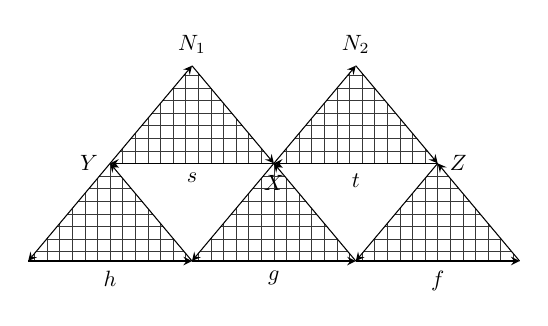
\begin{tikzpicture}[>=stealth,line width=.38pt,scale=.80,transform shape]
    \coordinate (Y)  at (0,0);
    \coordinate (X)  at (2.6,0);
    \coordinate (Z)  at (5.2,0);
    \coordinate (N1) at (1.3,1.55);
    \coordinate (N2) at (3.9,1.55);
    \coordinate (A)  at (-1.3,-1.55);
    \coordinate (Q1) at (1.3,-1.55);
    \coordinate (Q2) at (3.9,-1.55);
    \coordinate (B)  at (6.5,-1.55);

    \VerdierHatchTriangle{Y}{N1}{X}
    \VerdierHatchTriangle{X}{N2}{Z}
    \VerdierHatchTriangle{Y}{A}{Q1}
    \VerdierHatchTriangle{X}{Q1}{Q2}
    \VerdierHatchTriangle{Z}{Q2}{B}

    \draw[->] (Y) -- (N1);
    \draw[->] (N1) -- (X);
    \draw[->] (X) -- node[below=1pt] {$s$} (Y);
    \draw[->] (X) -- (N2);
    \draw[->] (N2) -- (Z);
    \draw[->] (Z) -- node[below=1pt] {$t$} (X);

    \draw[->] (Y) -- (A);
    \draw[->] (A) -- node[below=1pt] {$h$} (Q1);
    \draw[->] (Q1) -- (Y);
    \draw[->] (X) -- (Q1);
    \draw[->] (Q1) -- node[below=1pt] {$g$} (Q2);
    \draw[->] (Q2) -- (X);
    \draw[->] (Z) -- (Q2);
    \draw[->] (Q2) -- node[below=1pt] {$f$} (B);
    \draw[->] (B) -- (Z);

    \node[left=2pt]  at (Y)  {$Y$};
    \node[below=2pt] at (X)  {$X$};
    \node[right=2pt] at (Z)  {$Z$};
    \node[above=2pt] at (N1) {$N_1$};
    \node[above=2pt] at (N2) {$N_2$};
  \end{tikzpicture}
  \quad ,
\end{center}

\VerdierSemanticAnchor{ch2-2-1-13-diagram-interpretation}
\noindent ここで $N_1$ と $N_2$ は $\mathcal D'$ の対象であり、網掛けされた
五つの三角は完全三角、網掛けされていない二つの三角は可換である。

\VerdierSemanticAnchor{ch2-2-1-13-shifted-zero}
したがって $s[1]t=0$ (1.2.2)。
\VerdierSemanticAnchor{ch2-2-1-13-shifted-membership}%
さらに SM1)、SM5) により、射 $s[1]t$ は $S(\mathcal D')$ に属する。

\VerdierSemanticAnchor{ch2-2-1-13-split-triangle}
ゆえに $N$ が $\mathcal D'$ の対象であるような形
$(Z,Y[2],N,0,u,v)$ の完全三角が存在する。
\VerdierSemanticAnchor{ch2-2-1-13-direct-summand}%
(1.2.6)、TRII により $Y$ は $\mathcal D'$ のある対象の直和因子である。
\VerdierSemanticAnchor{ch2-2-1-13-y-in-dprime}%
よって $Y$ は $\mathcal D'$ の対象と同型である。

\VerdierSemanticAnchor{ch2-2-1-13-s-triangle}
(1.2.4)、$\mathcal D'$ が $\mathcal D$ の三角部分圏であること、および完全三角

\begin{center}
  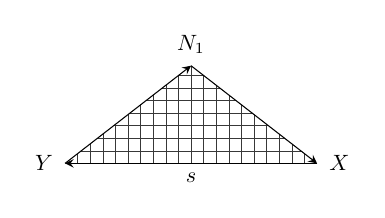
\begin{tikzpicture}[>=stealth,line width=.38pt,scale=.80,transform shape]
    \coordinate (Y)  at (-2,0);
    \coordinate (X)  at (2,0);
    \coordinate (N1) at (0,1.55);
    \VerdierHatchTriangle{Y}{N1}{X}
    \draw[->] (Y) -- (N1);
    \draw[->] (N1) -- (X);
    \draw[->] (X) -- node[below=1pt] {$s$} (Y);
    \node[left=2pt]  at (Y)  {$Y$};
    \node[right=2pt] at (X)  {$X$};
    \node[above=2pt] at (N1) {$N_1$};
  \end{tikzpicture}
\end{center}

\VerdierSemanticAnchor{ch2-2-1-13-g-membership}
\noindent から、$X$ が $\mathcal D'$ の対象と同型であると分かる。したがって
射 $g$ は $S(\mathcal D')$ に属する。

\VerdierSemanticAnchor{ch2-2-1-14}
\medskip
\noindent\textbf{2.1.14.}\quad
\VerdierSemanticAnchor{ch2-2-1-14-saturation-direction}%
\emph{$S(\mathcal D')$ が飽和ならば $\mathcal D'$ は飽和である。}

\VerdierSemanticAnchor{ch2-2-1-14-direct-summand-setup}
$X$ を $\mathcal D'$ のある対象の直和因子とする。
\VerdierSemanticAnchor{ch2-2-1-14-first-triangle}%
(1.2.6)、TRII により、$N$ が $\mathcal D'$ の対象であるような完全三角
$(X,Y,N,0,u,v)$ が存在する。
\VerdierSemanticAnchor{ch2-2-1-14-zero-morphism}%
したがって零射 $X\to Y$ は $S(\mathcal D')$ に属する。

\VerdierSemanticAnchor{ch2-2-1-14-sm4-application}
三射 $0\to X\to 0\to Y$ に SM4) を適用する。
\VerdierSemanticAnchor{ch2-2-1-14-x-zero-membership}%
すると射 $X\to 0$ は $S(\mathcal D')$ に属する。

\VerdierSemanticAnchor{ch2-2-1-14-second-triangle}
ゆえに $N$ が $\mathcal D'$ の対象であるような完全三角
$(X,0,N,0,0,i)$ が存在する。
\VerdierSemanticAnchor{ch2-2-1-14-shift-isomorphism}%
したがって射 $N\xrightarrow{i}X[1]$ は同型で、$X$ は $N[-1]$ と同型であり、
後者は $\mathcal D'$ の対象である。

\VerdierSemanticAnchor{ch2-2-1-14-proposition-complete}
これで命題 (2.1.8) の証明が完了した。

\VerdierSemanticAnchor{ch2-2-1-14-p134-boundary}
\endgroup
